\chapter{Hearing Aids}

%DONE
\section{Introduction}
\paragraph{}Hearing aids, quite simply, are prescribed to help listeners hear desired sounds in their everyday listening environments.  For most people who are fit with hearing aids, these desired sounds are primarily speech, so the main goal for wearing hearing aids is to restore one's ability to hear and understand speech.  However, one can imagine that speech is not the most desired signal to restore in all cases.  Take, for example, the case of a musician who needs to strain to hear particular instruments or frequencies.  In the musician's case, hearing loss may affect one's ability to perform his instrument, and it is quite conceivable for this person that restoring music perception ought to take priority over restoring speech perception.  Additionally, two people with the same audiogram may have vastly different tolerances for loud sounds and very different speech in noise outcomes.  Prescribing the same amount of amplification for these two people is bound to be a poor strategy.  The underlying theme here, is that there is not a one-fits-all solution when prescribing hearing aids, as every individual has their own needs.  For this very reason, it is common for hearing aid wearers to require one or several adjustments to their hearing aid fitting; the general best practice is to start off with an average best fit, and then perform one or several adjustments over the course of weeks or months to optimize an individual fitting, based on the patient's feedback.

Hearing aids are tasked with the difficult problem of amplifying sound just enough to restore speech intelligibility, while suppressing unwanted sounds (i.e. noise), for which the definition varies from person to person.  Hearing aids do not do a perfect job of restoring hearing back to normal, and there are still many returns for refund on hearing aids and hearing aids sitting unused in dresser drawers \cite{Kochkin2010b}.  Thus, there is much room for improvements to hearing aid technology.  The industry is on the right track, as hearing aid satisfaction has been slowly increasing \cite{Kochkin2010a}.

Three decades ago, in the 1980's, most hearing aids were linear, meaning that an equal amount of amplification was given to an input signal regardless of the level of the incoming input signal.  Once hearing science began to unravel and understand the issue of loudness recruitment (rapid growth of loudness in hearing-impaired subjects), compression was added to hearing instruments in order to amplify soft sounds more than loud sounds.  As hearing science progresses, common signal processing techniques will be added to hearing aids, with the hope of steadily increasing hearing aid satisfaction.

%DONE
\subsection{Physical Components}
\paragraph{}A hearing aid is made up of one or several small microphones, a battery, a speaker (often called a receiver), internal components which alter the original auditory signal, and a shell which houses all of these components in a small space.  An incoming acoustic signal is picked up by the microphone and transduced into electricity, which is then altered in some way by the internal components (the signal is generally split into different frequency channels, and given amplification proportional to the amount of hearing loss in each channel), and finally the speaker transduces the signal back into a sound pressure wave in the ear canal.

There have been considerable advances in hearing aid technology over the past couple decades, most dramatically in the way that sound is processed, amplified, and compressed.  In the early 1980's, all hearing aids were analog, meaning that physical transistors and other electrical components acted as the amplifiers, filters, and compressors.  Modern hearing aids, however, are essentially all digital, meaning that they all have digital signal processors (DSPs).  Unlike analog hearing aids, which alter the signal electrically with electrical components, digital hearing aids turn the acoustic signal into a string of numbers with an analog-to-digital converter, alter the signal mathematically with the DSP, and turn the signal back into sound with a digital-to-analog converter.  DSPs offer much more flexibility in the way of programming hearing aids and implementing more advanced signal processing algorithms, which has resulted in an explosion of features that are starting to become standard in modern hearing aids.

%DONE
\subsection{Features}
\paragraph{}Many technologies found on modern day hearing aids have existed for decades in one form or another, such as directional microphones, but it is only with the advent of DSPs that these technologies have been able to be exploited in order to improve hearing aid outcomes.

As mentioned previously, digital hearing aids are programmable.  Several programs can be installed on a single hearing aid (one for speech in quiet, one for music, etc.), and the user can change programs by pressing a button on the hearing aid, or by using a remote control.  Many modern hearing aids automatically adapt to their environments, switching between programs depending on the acoustic input.

Directional microphones are either implemented as one or several microphones, and are the only hearing aid technology that have been shown to improve speech intelligibility in noise, when used in optimal settings \cite{McCreery2012}.  Some newer directional microphone technologies track the location of the noise source and change their polar plot accordingly (adaptive directionality).

Noise reduction is another signal processing technique that is commonly seen on modern hearing aids.  \citeA{Plomp1983} discovered that noise-like stimuli have different temporal/envelope properties than speech-like stimuli, in that the rate of modulation of noise-like stimuli tends to be higher than speech, and the depth of modulation tends to be lower than speech.  Once this discovery was made, hearing aid algorithm designers exploited these differing characteristics between speech and noise, creating noise reduction schemes which reduced amplification in frequency channels where speech was statistically unlikely to be present.  In modern hearing aids, there are many different implementations of noise reduction \cite{Bentler2006}.  One problem with noise reduction is that everyone's definition of noise varies, so a noise reduction system that works well for one person will not necessarily work well for another person.  In a review of many different clinical studies investigating noise reduction, it was found that noise reduction does not improve or degrade speech understanding \cite{McCreery2012}.  Despite the lack of evidence for noise reduction improving speech intelligibility, there is emerging evidence that it can reduce cognitive effort \cite{Sarampalis2009}, thereby improving hearing aid fitting outcomes.

Similar to some other audio applications, one pervasive engineering problem with hearing aids is the problem of feedback.  With the microphone and speaker placed so close in proximity, and the near impossibility of forming a perfect seal with the ear canal, it is very difficult to prevent sound emanating from the receiver from leaking out of the ear canal and back into the microphone, creating a feedback loop.  One workaround that the industry has devised is to equip hearing aids with feedback cancellation algorithms.  The most popular forms of feedback cancellation work by detecting tonal stimuli, and subsequently reducing amplification in the frequency region(s) containing the tonal stimuli by using a notch filter, or by adding a signal which is opposite in phase to the feedback signal \cite{Parsa2006}.  Although feedback cancellers work well to suppress feedback, sometimes, for tonal sounds, the feedback canceller can produce what are called entrainment artifacts.  Entrainment artifacts are perceived as an additional tone or echo added in by the feedback canceller in order to attempt to cancel out a feedback-like signal.  Entrainment can even occur with non-feedback, tonal-like stimuli, such as a musical instrument, or alarms and beeps.

Another feature which has existed for some time but is just now becoming commonplace, is known as frequency lowering.  The main concept behind this technology is to shift higher frequency speech information to lower frequencies, where hearing loss is generally less severe.  As mentioned in a previous section, most hearing losses are greater in extent in the high frequencies; sometimes it is challenging to provide enough amplification in these regions in order to restore speech cues, and frequency lowering addresses this problem by shifting speech cues to lower frequencies that cannot be restored in the higher frequencies.  In some cases, amplification in regions with severe hair cell loss can even decrease speech intelligibility in quiet \cite{Vickers2001}.  Other studies have found high frequency amplification not to be detrimental to speech intelligibility \cite{Cox2012}.  Either way, there is evidence that frequency lowering may help restore speech intelligibility \cite{Simpson2005, Glista2009}.

As DSPs become faster and increase in memory capacity, the number of hearing aid features will continue to grow.  Audiologists and hearing instrument specialists are in some sense forced to keep pace with the advent of new features, or they risk falling behind the curve, potentially losing business as a result.  There is a need for hearing aid algorithms to build in these features implicitly, which would make it easier for audiologists and hearing instrument specialists to keep up with new technologies, therefore simplifying the fitting process both for the hearing practitioners as well as the patients.

%DONE
\section{Hearing Aid Prescriptions}
\subsection{Overview}
\paragraph{}As discussed in the previous chapter, the first step in programming a hearing aid is to collect an audiogram for a patient.  With the audiogram, a prescription can be generated for a given hearing aid using the hearing aid manufacturer's fitting software.  Prescription gain formulas differ across hearing aid manufacturers, but most are generally derived from either the National Acoustic Laboratories (NAL) formulas \cite{Byrne1986, Byrne1990, Dillon1999, Keidser2011}, or the Desired Sensation Level (DSL) formulas \cite{Cornelisse1995, Scollie2005}, which are two families of empirically derived prescription formulas that have been developed over the past couple decades.  There have been many revisions to the NAL and DSL fitting formulas over the years, which first started out as linear prescriptions, and have since been revised to be nonlinear prescriptions in order to accommodate compression, a common signal processing technique found on essentially all modern hearing aids.  Most fitting software packages allow the clinician to select NAL or DSL directly, in addition to the manufacturer's prescription.

A hearing aid prescription specifies the target amount of gain that the hearing aid ought to prescribe for a given audiometric loss, as a function of frequency and intensity.  Decades of research have went into optimizing the amount of gain as a function of frequency and intensity for the full range of hearing losses.  Usually, 3 target output curves are plotted on the fitting graph; one for soft speech, one for average speech, and one for loud speech.  Figure 2.1 illustrates an example of a particular fitting software's target curves.  In Figure 2.1, the red lines plot the target gain curves as a function of frequency, and the blue lines plot the estimated gain delivered by the hearing aid.  In this particular example, the blue lines are lower than the red lines on the y-axis, meaning that the estimated gain delivered by the hearing aid is less than that prescribed.  The highest curve for each color corresponds to an input of 40 dB, the middle curve is for an input of 65 dB, and the bottom curve is for an input of 90 dB.  The fact that the soft, average, and loud inputs have different curves indicates that compression is being prescribed (low level sounds require more gain than high level sounds, in order to compensate for the loss of OHCs, which effectively amplify low level sounds).  Using the software, clinicians can adjust the amount of gain as a function of frequency.

\begin{figure}
\begin{center}
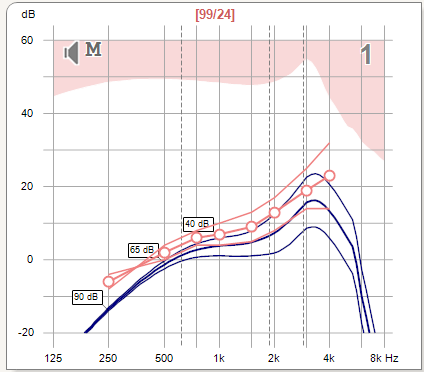
\includegraphics[height=3in]{chap2-target-curves.png} \\
\caption[Hearing aid target curves]{Target curves for a single hearing aid.  The red lines plot the amount of gain prescribed by the fitting software, for soft speech (40 dB), average speech (65 dB), and loud speech (90 dB).  The blue lines plot the estimated gain of the hearing aid as a function of frequency.  For this particular fitting, the estimated gain is less than the target curves prescribe, meaning that the hearing aid is under-fit.  Compression can be seen, in that the soft speech gain curves are giving more gain than the average and loud speech gain curves.}
\label{ch2-target-curves}
\end{center}
\end{figure}

The focus of generally all hearing aid prescription formulas is to normalize loudness in individual frequency channels, or across frequency channels, while maximizing speech intelligibility.  Wide dynamic range compression (WDRC), which can be implemented as one out of many prescription formulas, is a nonlinear amplification strategy used to map the larger dynamic range of normal hearing onto the smaller dynamic range of a hearing-impaired person, as illustrated in Figure 2.2.  The essence of WDRC is that it gives more amplification to quiet sounds than to loud sounds, reducing the amount of loudness that would result from amplifying loud sounds, while increasing the audibility of soft sounds (mimicking the compressive nonlinearity of the basilar membrane for normal hearing).  Some studies have demonstrated speech intelligibility benefits when using a WDRC scheme in place of a linear gain strategy \cite{Jenstad1999, Humes1999}.  The hearing aid comparison study reported on in this thesis used WDRC as the standard for comparison, given its widespread acceptance, accessibility, and influence on the hearing aid industry.

\begin{figure}
\begin{center}
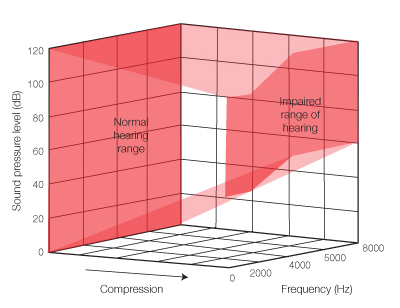
\includegraphics[height=3in]{chap2-dynamic-range.png} \\
\caption[WDRC and dynamic range]{WDRC and dynamic range.  People who are hearing-impaired have a reduced dynamic range (soft sounds are inaudible, but loud sounds are just as loud as with normal hearing). WDRC applies amplification in different frequency bands independently, and maps the dynamic range of normal hearing onto the dynamic range of impaired hearing.  (Retrieved June 1, 2013, from: http://www.gnresound.ca/professionals/technology-and-innovation/surround-sound-by-resound/wide-dynamic-range-compression) }
\label{ch2-dynamic-range}
\end{center}
\end{figure}

%DONE
\subsection{Problems With Prescription Formulas}
\paragraph{}There are two main problems with current prescription formulas, despite the success that these formulas have had with restoring normal loudness perception.

The first problem is that WDRC treats each frequency channel independently, largely ignoring frequency by frequency relationships, which exist in most complex sounds.  A complex sound is any sound that is made up of more than one frequency, and the vast majority of sounds encountered in everyday environments are complex.  The consequence of ignoring frequency by frequency interactions in an amplification algorithm is that distortion is added to the original signal by altering frequency-specific interactions.  Frequency-specific interactions carry important information, and when altered the result can be a reduction in speech intelligibility and sound quality.  One example comes from a study by \citeA{Kiefte2005}, who showed that altering the intensity relationships of vowel formants reduces vowel intelligibility.  Music offers another example of how ignoring frequency by frequency interactions can degrade intelligibility or quality.  When a musical instrument sounds a note, a fundamental frequency is generated, as well as several harmonics produced at integer multiples of the fundamental frequency.  Timbre, the musical quality that allows one to differentiate one musical sound from another with the same pitch, loudness, and duration, depends on attack times, the spectral energy distribution of the instrument, and the temporal envelope synchronicity across partials \cite{Grey1977}.  Applying amplification unequally across all frequency bands distorts the spectral energy distribution, and obscures the timbre of an instrument, especially when compression is activated.  Such a distortion in timbre alters the information contained in the musical passage, and can affect the perceived quality of this music.  Given how a musical signal's timbre can be altered by applying unequal amplification across frequencies, it follows that other timbres are also likely modified (e.g. vocal timbres).

The second problem with standard prescription formulas is that they only attempt to optimize one kind of signal; speech.  Optimizing loudness for speech does not necessarily optimize loudness for other complex sounds.  For example, while the correlation between the physical and perceptual intensity of speech is high, for some musical instruments it is low (bass, cello), especially for instruments that have multiple harmonics which fall in the same critical band, resulting in less loudness summation \cite{Chasin2004}.  Additionally, sound localization is an important ability that is enabled by having two ears, pinna filtering, and complex signal processing in the auditory system, and is performed by calculating interaural time and level differences (ITD, ILD) between the ears \cite{Middlebrooks1991}.  Standard prescription formulas do not consider sound localization, and ITD and ILD cues could be distorted by these formulas.  In fact, several studies have demonstrated that hearing aids actually impair sound localization abilities relative to wearing no hearing aids at all \cite{Noble1990, VandenBogaert2006, Keidser2006}, so there is likely room for improvement to current hearing aid prescriptions in restoring these cues for sound localization.

Clearly, there exists a need for a single hearing aid algorithm which is capable of restoring as many of the abilities that normal hearing listeners take for granted, such as accurate speech intelligibility in quiet and noise, high fidelity music perception, and proper sound localization.  The purpose of this thesis is to investigate a novel hearing aid called the Neuro-Compensator (NC), which exploits a neural-based amplification algorithm \cite{Bondy2004} that could potentially provide many benefits that other hearing aids fail to provide.  At present, there is anecdotal evidence of improvements in speech intelligibility, music perception, and sound localization abilities in users fit with the NC.

\section{Neuro-Compensator}
\paragraph{}The NC uses neurophysiological models of the normal and impaired auditory periphery \cite{Bruce2003}, which are used to  estimate auditory nerve output for a given sound input.  The output of the models for a given stimulus are plotted as neurograms, which are essentially plots of neural spiking rates as a function of AN fiber CFs.  The block diagram in the left panel of Figure 2.3 illustrates the basic idea of the NC.  An input to a normally hearing ear (X) is processed by the normal auditory periphery (H) and responds with normal neural output (Y).  In a damaged auditory periphery (one with SNHL), when the same input (X) is presented to the ear, the damaged auditory periphery (\^{H}) does not recreate normal neural output but rather results in a distorted neural output (\^{Y}).  By pre-processing the input (X) to the damaged auditory periphery (\^{H}) with the NC algorithm, perceptual distortions are minimized by recreating a more normal neural output (Y).

\begin{figure}[ht]
\begin{center}
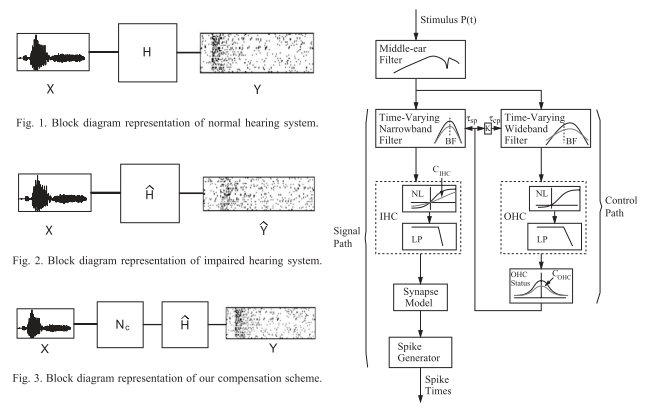
\includegraphics[]{chap2-NC-block-diagrams.png} \\
\caption[Neuro-Compensator concept]{The Neuro-Compensator concept.  \emph{Left:} The Neuro-Compensator block preprocesses an input acoustic waveform, such that when the processed input is fed into a damaged auditory nerve (\^{H}), a near normal auditory nerve output (Y) is produced.  \emph{Right:} Schematics of the \citeA{Bruce2003} auditory nerve model.  (Both figures were reprinted from \citeA{Bondy2004}). }
\label{ch2-NC-block-diagrams}
\end{center}
\end{figure}
	
The details of the auditory periphery model can be seen in the right panel of Figure 2.3.  First, the input is processed by the \citeA{Wiener1946} head related transfer function and the middle ear filter.  The control path (OHCs) then modulates the signal path (IHCs) with a wideband, nonlinear, time-varying band-pass filter and OHC nonlinearity and a low-pass filter, controlling the behaviour of the narrowband signal path BM filter.  The signal path then mimics traveling wave and filter properties of the BM, and generates spikes in the auditory nerve with spontaneous and driven activity using spike generation and auditory nerve refractoriness.  The \citeA{Bruce2003} model effectively models many nonlinear characteristics of the cochlea, such as the compressive input-output response of the BM, masking effects like two-tone suppression, synchrony capture in the normal and damaged ear, and shifted tuning curves with OHC damage.

The NC is fit to a particular hearing loss by supplying an audiogram, and training adjustable weights which are present in the NC gain term, for a corpus of training samples (speech).  The gain term for the NC is based upon a spectral contrast enhancement scheme proposed by \citeA{Schwartz2001}.  The gain prescribed for a particular frequency channel depends on the output power in the channel ($P_i$), normalized by a weighted sum of power in the other frequency channels ($P_j$) multiplied by the trainable weights ($v_{ij}$), plus a constant ($\sigma$) to prevent gain from exceeding a certain limit (see Equation 2.1, below).

\begin{equation}
G_i = \frac{P_i}{\sum_{j} (v_{ij} P_j) + \sigma}
\end{equation}

On each iteration of the training algorithm, the output of the normal and aided impaired auditory nerve models are compared, and the weights in the NC gain terms ($v_{ij}$'s in the formula) are adjusted using a modified version of a stochastic optimization algorithm called Alopex (the original version of Alopex was proposed by \citeA{Unnikrishnan1994}).  Currently, the error metric used to compute the difference between the normal and aided-impaired neurograms is a simple absolute difference between the two neurograms.  Over several training iterations, the overall error between neurograms is minimized and an optimal set of weights ($v_{ij}$) in the gain term are obtained for a given individual.  The logic is that the optimal set of weights will reduce perceptual distortions and perhaps restore some nonlinear behaviour of the cochlea because the compensated neural output is restored to be as close to normal as possible. 